\documentclass[12pt]{extarticle}
\usepackage[a4paper,margin=2.5cm]{geometry}
\usepackage{lmodern}
\usepackage{microtype}
\usepackage{parskip}
\usepackage{amssymb}
\usepackage{amsmath}
\usepackage{amsfonts} 
\usepackage{hyperref}
\usepackage{graphicx}
\usepackage{listings}
\usepackage[T1]{fontenc}
\usepackage[utf8]{inputenc}
\usepackage[spanish]{babel}
\usepackage{minted}
\usepackage{graphicx}
\graphicspath{ {./imagenes/} }

\author{Mateo Ziffer}
\title{Apunte Final PLP}

% https://tex.stackexchange.com/questions/60209/how-to-add-an-extra-level-of-sections-with-headings-below-subsubsection
\setcounter{secnumdepth}{5}
\setcounter{tocdepth}{5}
\makeatletter
\newcommand\subsubsubsection{\@startsection{paragraph}{4}{\z@}{-2.5ex\@plus -1ex \@minus -.25ex}{1.25ex \@plus .25ex}{\normalfont\normalsize\bfseries}}
\newcommand\subsubsubsubsection{\@startsection{subparagraph}{5}{\z@}{-2.5ex\@plus -1ex \@minus -.25ex}{1.25ex \@plus .25ex}{\normalfont\normalsize\bfseries}}
\makeatother

\def\propiedad{\underline{Prop:} }
\def\definicion{\newline\underline{Def:} }
\def\demostracion{\underline{Demo:} }
\def\teorema{\underline{Teo:} }
\def\corolario{\underline{Coro:} }
\def\observacion{\underline{Obs:} }
\def\ejemplo{\textit{\underline{Ejemplo} }}
\def\ejercicio{\textit{\underline{Ejercicio} }}

\def\flecha{$\rightarrow$}
\def\eval{$\rightsquigarrow$}
\def\equ{\overset{?}{=}}
\def\True{\text{True}}
\def\False{\text{False}}
\def\Bool{\text{Bool}}
\newcommand\ifelse[3]{\text{if }#1\text{ then }#2\text{ else }#3}
\def\modelsM{\models_\mathcal{M}}

\def\ssspace{\space\space\space}

\newcommand\hsline[1]{\mintinline{hs}{#1}}

\newcommand\paratodo[2]{$\forall$\hsline{#1 :: #2}.}

\newcommand\regla[3]{$\frac{\text{#3}}{\text{#2}} \text{#1}$}

\newcommand\Regla[3]{\frac{\text{#3}}{\text{#2}} \text{#1}}

\begin{document}
\maketitle{}
\tableofcontents
\newpage \section{Introducción}
En esta sección escribiré algunas definiciones generales y el objetivo de la materia.
\definicion la \textit{programación} es el proceso de escribir instrucciones que una computadora puede ejecutar para resolver algún problema.
\definicion un \textit{programa} es una serie de instrucciones/definiciones que una computadora sigue para realizar una tarea específica.
\definicion un \textit{lenguaje de programación} es un formalismo artificial en el que se pueden describir compataciones.
\definicion un \textit{paradigma} es una marco filosófico y teórico de una escuela científica o disciplina en la que se formulan teorías, leyes y generalizaciones y se llevan a cabo experimentos que les dan sustento.
\definicion un \textit{paradigma de programación} es una marco filosófico y teórico en el que se formulan soluciones a problemas de naturaliza algorítmica. \\
Lo entendemos como un estilo de programación en el que se escriben soluciones a problemas en términos de algoritmos. \\

Estudiamos la gramática, semántica, pragmática e implementación de los lenguajes de programación.
\definicion la \textit{gramática} responde a ¿Qué frases son correctas?, establece el alfabeto, las palabras (o tokens), es decir, la secuencia válida de símbolos y la sintaxis, es decir, las secuencias de palabras que son frases legales.
\definicion la \textit{semántica} responde a ¿Qué significa una frase correcta?, estableciendole un significado a cada frase correcta.
\definicion la \textit{semántica} responde a ¿Qué significa una frase correcta?, estableciendole un significado a cada frase correcta.
\definicion la \textit{pragmática} responde a ¿Cómo usamos una frase significativa?. Las frases con el mismo significado pueden usarse de diferentes maneras, diferentes contextos pueden requerir frases más elegantes, eficientes, dialectales, etc.
\definicion la \textit{implementación} responde a ¿Cómo ejecutar una frase correcta, de manera que respetemos la semántica?. Es fundamentas para los diseñadores e implementadores del lenguaje, no necesariamente para el usuario (programador).

Hay tres apectos importantes de los lenguajes de programación: \\
\underline{Motivación} de la \textit{programación}: los lenguajes de programación tienen distintas características que permiten abordar un mismo problema de distintas ma los lenguajes de programación tienen distintas características que permiten abordar un mismo problema de distintas maneras. \\
\underline{Motivación} de la \textit{semántica}: probar teoremas sobre el comportamiento de los programas, para darles significado matemático y poder confiar en que hace lo que queremos, en AED vimos como hacerlo con triplas de Hoare, pero en PLP veremos otras maneras de dar semántica. \\
\underline{Motivación:} la \textit{implementación}: una computadora física ejecuta programas escritos en un lenguaje, el código máquina, pero necesita poder ejecutar programas escritos en otros lenguajes, a través de la interpretación, el chequeo e inferencia de tipos y la compilación. \\

\section{Deducción natural, lógica proposicional y lógica de primer orden}
\subsection{Sistema deductivo}
Queremos podes hacer afirmaciones matemáticamente precisas sobre programas en distintos lenguajes de programación.
\definicion sistema deductivo: sirve para razonar acerca de juicios. Dado un conjunto de axiomas y reglas de inferencia que tienen la siguiente estructura: \\

\regla{$\langle$nombre del axioma$\rangle$}{
  $\langle$axioma$\rangle$
}{}
\regla{$\langle$nombre de la regla$\rangle$}{
  $\langle$conclusión$\rangle$
}{
  $\langle$premisa$_0\rangle$
  $\langle$premisa$_1\rangle$
  ...
  $\langle$premisa$_n\rangle$
} \\ \\
\definicion axioma. afirmacion basica que se asuma como verdadera
\definicion regla de inferencia. permite derivar afirmaciones (teoremas) a partir de axiomas y otras afirmaciones \\
\observacion un axioma es una regla de inferencia sin premisas

Las premisas son condiciones suficientes para la conclusión.
\definicion derivación. Procedimiento sistemático que permite construir una demostración, mostrando cómo una afirmación se deduce a partir de un conjunto de axiomas y reglas de inferencia.
\definicion arbol de derivacion. Representación gráfica de una derivación. Un árbol finito donde los nodos representan afirmaciones, la raóz es la afirmación que se quiere probar y las ramas representan las reglas de inferencias que conectan a las afirmaciones. Parte de ciertas premisas (hojas) y llega a una conclusión (raíz).
\definicion una afirmación es derivable si existe alguna derivación sin premisas que la tiene como conclusión.

\subsection{Lógica proposicional}

\subsubsection{Sintaxis}
Suponesos un conjunto infinito de variables proposicionales $\mathcal{P} = \{P, Q, R, ...\}$. Las fórmulas bien formadas (fbf) de la lógica proposicional se construyen inductivamente según las siguientes reglas:

\begin{itemize}
\itemsep-0.35em 
\item cualquier variable proposicional es una fórmula.
\item $\bot$ es una fórmula.
\item si $\tau$ es una fórmula, entonces $\neg\tau$ es una fórmula.
\item si $\tau$ y $\sigma$ son fórmulas, entonces $(\tau \land \sigma)$, $(\tau \lor \sigma)$ y $(\tau \Rightarrow \sigma)$ son fórmulas.
\end{itemize}
Como sistema deductivo, la afirmación X FORM denota que X es una fórmula de la lógica proposicional.
$$
\Regla{FP\ssspace}{$P$ FORM}{$P \in \mathcal{P}$}
\Regla{F$\bot$\ssspace}{$\bot$ FORM}{}
\Regla{F$\neg$\ssspace}{$\neg \tau$ FORM}{$\tau$ FORM}
$$
$$
\Regla{F$\land$\ssspace}{$\tau \land \sigma$ FORM}{$\tau$ FORM \ssspace $\sigma$ FORM}
\Regla{F$\lor$\ssspace}{$\tau \lor \sigma$ FORM}{$\tau$ FORM \ssspace $\sigma$ FORM}
\Regla{F$\Rightarrow$}{$\tau \Rightarrow \sigma$ FORM}{$\tau$ FORM \ssspace $\sigma$ FORM}
$$

Usualmente no vamos a definir la sintaxis de lenguajes a través de sistemas deductivos, vamos a escribirlos de maneras abreviadas, usando gramáticas.
\definicion las fórmulas son las expresiones que se pueden generar a partir de la siguiente gramática:
$$ \tau,\sigma,\rho ::= P | \bot | (\tau \land \sigma) | (\tau \lor \sigma) | (\tau \Rightarrow \sigma) | \neg \tau $$

\observacion las gramáticas definen sistemas deductivos de manera abreviada. Una expresión $\tau$ se puede generar a partir de la gramática de arriba sii el juicio $\tau FORM $ es derivable en el sistema anterior.

Por convenciones de notación, omitimos paréntesis más externos y la implicación es asociativa a derecha, pero cuidado con los otros conectivos que no son conmutativos ni asociativos.

\subsubsection{Semántica}
Recordemos, la \textit{semántica} responde a ¿Qué significa una frase correcta?, estableciendole un significado a cada frase correcta.
\definicion una valuación es una función $\mathcal{P} \rightarrow \{V,F\}$ que asigna valores de verdad a las variables proposicionales.
\definicion una valuación $v$ satisface una fórmula $\tau$ si $v \models \tau$, donde
\begin{align*}
  v \models P \text{ sii }& v(P) = V \\
  v \models \tau \land \sigma \text{ sii }& v \models \tau \text { y } v \models \sigma \\
  v \models \tau \lor \sigma \text{ sii }& v \models \tau \text{ o } v \models \sigma \\
  v \models \tau \Rightarrow \sigma \text{ sii }& v \not\models \tau \text{ o } v \models \sigma \\
  v \models \neg \tau \text{ sii }& v \not\models \tau
\end{align*}

\observacion $v \models \bot$ nunca vale.
\definicion un contexto $\Gamma$ es un conjunto finito de fórmulas.
\definicion una valuación $v$ satisface un contexto $\Gamma$ ($v \models \Gamma$) sii $v$ satisface a todas las fórmulas de $\Gamma$. Nota: toda valuación satisface al contexto vacío.
\definicion una fórmula $\tau$ es consecuencia lógica (o consecuencia semántica) de un conjunto $\Gamma$ ($\Gamma \models \tau$) sii cualquier valuación $v$ que satisface a $\Gamma$ también satisface a $\tau$.

Hay varios problemas con un enfoque puramente semántica, por eso vamos a definir un sistema deductivo.

\subsection{Deducción natural}
Es un sistema deductivo, pero existe otros. Trabaja con afirmaciones de la forma.
{\Large $$\underbrace{\Gamma}_{\text{hipótesis}} \vdash \underbrace{\tau}_{\text{tesis}}$$ }
A estas afirmaciones las denominamos juicios. Informalmente, un juicio afirma que a partir de las hipótesis en el contexto $\Gamma$ es posible deducir la fórmula de la tesis.

\subsubsection{Deducción natural intuicionista (NJ)}

$$
\Regla{ax\ssspace}{$\Gamma, \tau \vdash \tau$}{}
\Regla{$\bot_e$\ssspace}{$\Gamma \vdash \tau$}{$\Gamma \vdash \bot$}
\Regla{$\neg_i$\ssspace}{$\Gamma \vdash \neg \tau$}{$\Gamma, \tau \vdash \bot$}
\Regla{$\neg_e$}{$\Gamma \vdash \bot$}{$\Gamma \vdash \tau$ \ssspace $\Gamma \vdash \neg \tau$}
$$

$$
\Regla{$\land_i$\ssspace}{$\Gamma \vdash \tau \land \sigma$}{$\Gamma \vdash \tau$ \ssspace $\Gamma \vdash \sigma$}
\Regla{$\land_{e_1}$\ssspace}{$\Gamma \vdash \tau$}{$\Gamma \vdash \tau \land \sigma$}
\Regla{$\land_{e_2}$}{$\Gamma \vdash \sigma$}{$\Gamma \vdash \tau \land \sigma$}
$$

$$
\Regla{$\lor_{i_1}$\ssspace}{$\Gamma \vdash \tau \lor \sigma$}{$\Gamma \vdash \tau$}
\Regla{$\lor_{i_2}$\ssspace}{$\Gamma \vdash \tau \lor \sigma$}{$\Gamma \vdash \sigma$}
\Regla{$\lor_e$}{$\Gamma \vdash \rho$}{$\Gamma \vdash \tau \lor \sigma$ \ssspace $\Gamma, \tau \vdash \rho$ \ssspace $\Gamma, \sigma \vdash \rho$}
$$

$$
\Regla{$\Rightarrow_i$\ssspace}{$\Gamma \vdash \tau \Rightarrow \sigma$}{$\Gamma, \tau \vdash \sigma$}
\Regla{$\Rightarrow_e$\ssspace}{$\Gamma \vdash \sigma$}{$\Gamma \vdash \tau \Rightarrow \sigma$ \ssspace $\Gamma \vdash \tau$}
$$

\teorema (debilitamento) Si $\Gamma \vdash \tau$ es derivable, entonces $\Gamma, \sigma \vdash \tau$ es derivable.
$$ \Regla{W}{$\Gamma, \sigma \vdash \tau$}{$\Gamma \vdash \tau$} $$

Se puede demostrar por inducción estructural en la derivación.

\textit{Reglas derivadas}
$$
\Regla{MT\ssspace}{$\Gamma \vdash \neg \tau$}{$\Gamma \vdash \tau \Rightarrow \sigma$ \ssspace $\Gamma \vdash \neg \sigma$}
\Regla{$\neg \neg_i$}{$\Gamma \vdash \neg \neg \tau$}{$\Gamma \vdash \tau$}
$$

\subsubsection{Deducción natural clásica (NK)}
NK extiende a NJ con principios de razonamiento clásicos. Si un juicio es derivable en NJ, también es derivable en NK. NJ es más restrictiva. Para hacer matemática, comúnmente usamos lógica clásica. Las derivaciones NJ se pueden entender como programas. NJ es la base de un lenguaje de programación funcional.
$$
\Regla{$\neg \neg_e$ \ssspace}{$\Gamma \vdash \tau$}{$\Gamma \vdash \neg \neg \tau$}
\Regla{LEM\ssspace}{$\Gamma \vdash \tau \lor \neg \tau$}{}
\Regla{PBC}{$\Gamma \vdash \tau$}{$\Gamma, \neg \tau \vdash \bot$}
$$

Con agregar una de las tres reglas pues de cualquiera se pueden deducir las otras.

\teorema (Corrección y completitud). Son equivalentes $\Gamma \vdash \tau$ es derivable en NK y $\Gamma \models \tau$.

\subsection{Unificación}
Suponemos un conjunto finito de constructores de tipos. Los tipos se forman usando incógnitas y constructores. $\tau ::= X_n | C(\tau_1, ..., \tau_n)$. La unificación es el problema de resolver sistemas de ecuaciones entre tipos con incógnitas.

Una sustitución es una función que a cada incógnita le asocia un tipo. Notamos $\{X_(k_1) := \tau_1, ..., X_(k_n) := \tau_n\}$ a la sustitución $S$ tq $S(X_(k_i)) = \tau_i$ para cada $1 \leq i \leq n$ y $S(X_k) = X_i$ para cualquier otra incógnita. Si $\tau$ es un tipos, escribimos $S(\tau)$ para el resultado de reemplazar cada incógnita de $\tau$ que le otorga $S$.

El problema de unificación es un conjunto finito $E$ de ecuaciones entre tipos que pueden involucrar incógnitas.
$$E = \{\tau_1 \equ \sigma_1,...,\tau_n \equ \sigma_n\}$$
El unificador para $E$ es una sustitución $S$ tq $S(\tau_1) = S(\sigma_1)$, ..., $S(\tau_n) = S(\sigma_n)$.

En general la solución al problema de unificación no es única (pueden haber infinitas). Una sustitución $S_A$ es más general que una sustitución $S_B$ si existe una sustitución $S_C$ tal que $S_B = S_C \circ S_A$. Es decir, $S_B$ se obtiene instanciando variables de $S_A$.

\textit{Algoritmo de unificación de Martelli-Montanari}
Dado un problema de unificación $E$, mientras $E \neq \empty$, se aplica sucesivamente alguna de las seis reglas. Esta puede resultar en una falla, de lo contrario, la regla es de la forma $E \rightarrow_S E'$. La resolución del problema $E$ se reduce a resolver otro problema $E'$ aplicando la sustitución $S$.

\begin{align*}
  \{X_n \equ X_n\} \cup E \overset{\text{Delete}}{\longrightarrow}& E \\
  \{C(\tau_1,...,\tau_n) \equ C(\sigma_1,...,\sigma_n)\} \cup E \overset{\text{Decompose}}{\longrightarrow}& \{\tau_1 \equ \sigma_1, ..., \tau_n \equ \sigma_n\} \cup E \\
  \{\tau \equ X_n\} \cup E \overset{\text{Swap}}{\longrightarrow}& \{X_n \equ \tau\} \cup E \\
  \{X_n \equ \tau\} \cup E \overset{\text{Elim}}{\longrightarrow}&_{\{X_n := \tau\}} E' = \{X_n := \tau\}(E) \text{si $X_n$ no ocurre en $\tau$}\\
  \{C(\tau_1,...,\tau_n) \equ C'(\sigma_1,...,\sigma_m)\} \cup E \overset{\text{Clash}}{\longrightarrow}& \text{falla si $C \neq C'$} \\
  \{X_n \equ \tau\} \cup E \overset{\text{Occurs-Check}}{\longrightarrow}& \text{falla si $X_n \neq \tau$ y $X_n$ ocurre en $\tau$}
\end{align*}

\teorema (Corrección)
El algoritmo termina para cualquier problema de unificación $E$. Si $E$ no tiene solución, el algoritmo llega a una falla. Si tiene solución, el algoritmo llega a $\empty$: $E = E_0 \rightarrow_{s_1} E_1 \rightarrow_{s_2} E_2 \rightarrow ... \rightarrow_{s_n} E_n = \empty$. Además, $S = S_n \circ ... \circ S_2 \circ S_1$ es un unificador para $E$. Además, dicho unificador es el más general posible (salvo renombre de incógnitas).

Notamos $mgu(E)$ al unificador más general de $E$, si existe.

\subsection{Lógica de primer orden}
La lógica proposicional permite razonar acerca de proposiciones, mientras que la lógica de primer orden permite razonar acerca de elementos sobre los que se predica, extendiendola con términos y cuantificadores.
\definicion un lenguaje de primer orden $\mathcal{L}$ está dado por un conjunto de símbolos de función $\mathcal{F} = \{f,g,h,...\}$ y un conjunto de símbolos de predicado $\mathcal{P} = {P,Q,R,...}$, cada símbolo y predicado con una aridad asociada $\geq 0$.

Suponemos fijado un lenguaje de primer orden $\mathcal{L}$ y un conjunto infinito numerable de variable $\mathcal{X} = \{X,Y,Z,...\}$.
  \definicion el conjunto $\mathcal{T}$ de términos se define por la siguiente gramática: $t ::= X | f(t_1,...,t_n)$.

Extendemos la gramática de las fórmulas en lógica proposicional y la extendemos a lógica de primer orden. \\
$\sigma ::= \mathcal{P}(t_1,...,t_n) | \bot | \sigma \Rightarrow \sigma | \sigma \land \sigma | \sigma \lor \sigma | \neg \sigma | \forall X. \sigma | \exists X. \sigma$

Una ocurrencia de una variable $X$ en una fórmula está ligada si está bajo el alcance de un cuantificador $\forall X / \exists X$ y libre si no. Dos fórmulas que sólo difieren en los nombres de las variables ligadas se consideran iguales.

Notamos $\sigma\{X := t\}$ a la sustitución de las ocurrencias libres de $X$ en la fórmula $\sigma$ por el término $t$, evitando la captura de variables.

\subsubsection{Deducción natural en LPO}
Se agregan reglas de introducción y eliminación para $\forall$ y $\exists$.

$$
\Regla{$\forall$E\ssspace}{$\Gamma \vdash \sigma\{X := t\}$}{$\Gamma \vdash \forall X. \sigma$}
\Regla{$\forall$I\ssspace}{$\Gamma \vdash \forall X. \sigma$}{$\Gamma \vdash \sigma$ $X \notin \text{fv}(\Gamma)$}
$$
$$
\Regla{$\exists$I\ssspace}{$\Gamma \vdash \exists X. \sigma$}{$\Gamma \vdash \sigma\{X := t\}$}
\Regla{$\exists$E\ssspace}{$\Gamma \vdash t$}{$\Gamma \vdash \exists X. \sigma$ $\Gamma, \sigma \vdash t$ $X \notin \text{fv}(\Gamma, t)$}
$$

\subsubsection{Semántica}
Suponemos fijado un lenguaje de primer orden $\mathcal{L}$.\definicion una estructura de primer orden es un par $\mathcal{M} = (M, I)$ donde $\mathcal{M}$ es un conjunto no vacío, llamado universo, $I$ es una función que le da una interpretación a cada símbolo, para cada símbolo de función $f$ de aridad $n$, $I(f): M^n \rightarrow M$, y para cada símbolo de predicado $P$ de aridad $n$, $I(P) \subseteq M^n$.

Suponemos fijada una estructura de primer orden $\mathcal{M} = (M,I)$.
\definicion una asignación es una funci
on que a cada variables le asigna un elemento del universo $a: \mathcal{X} \rightarrow M$.
\definicion cada término $t \in \mathcal{T}$ se interpreta como un elemento $a(t) \in M$.

Definimos una relación de satisfacción $a \models_\mathcal{M} \sigma$, representando que la asignación $a$ bajo la estructura $\mathcal{M}$ satisface la fórmula $\sigma$.
\begin{align*}
  &a \modelsM P(t_1,...,t_n) \text{ sii } (a(t_1),...,a(t_n)) \in I(P) \\
  &a \modelsM \sigma \land \tau \text{ sii } a \modelsM \sigma \text{ y } a \modelsM \tau \\
  &a \modelsM \sigma \lor \tau \text{ sii } a \modelsM \sigma \text{ o } a \modelsM \tau \\
  &a \modelsM \sigma \Rightarrow \tau \text{ sii } a \not\modelsM \sigma \text{ o } a \modelsM \tau \\
  &a \modelsM \neg \sigma \text{ sii } a \not\modelsM \sigma \\
  &a \modelsM \forall X. \sigma \text{ sii } a[X \mapsto m] \modelsM \sigma \text{ para todo } m \in M \\ 
  &a \modelsM \forall X. \sigma \text{ sii } a[X \mapsto m] \modelsM \sigma \text{ para algún } m \in M
\end{align*}
\definicion decimos que una fórmula $\sigma$ es
\begin{align*}
  &\text{Válida si } a \modelsM \sigma \text{ para toda } \mathcal{M}, a \\
  &\text{Inválida si } a \not\modelsM \sigma \text{ para alguna } \mathcal{M}, a \\
  &\text{Satisfactible si } a \modelsM \sigma \text{ para alguna } \mathcal{M}, a \\
  &\text{Insatisfactible si } a \modelsM \sigma \text{ para toda } \mathcal{M}, a
\end{align*}

\observacion sea $\sigma$ una fórmula,
\begin{align*}
  &\sigma \text{ es Válida sii } \sigma \text{ no es Inválida} \\
  &\sigma \text{ es Satisfactible sii } \sigma \text{ no es Insatisfactible} \\
  &\sigma \text{ es Válida sii } \neg\sigma \text{ es Insatisfactible} \\
  &\sigma \text{ es Satisfactible sii } \neg\sigma \text{ es Inválida}
\end{align*}

Una sentencia es una fórmula $\sigma$ sin variables libres. \\
Una teoría de primer orden es un conjunto de sentencias.
\definicion (Consistencia) Una teoría $\mathcal{T}$ es consistente si $\mathcal{T} \not\vdash \bot$.
\definicion (Modelo) Una estructura $\mathcal{M} = (M,I)$ es un modelo de una teoría $\mathcal{T}$ si vale $\modelsM \sigma$ para toda fórmula $\sigma \in \mathcal{T}$ (la asignación es irrelevante pues $\sigma$ es cerrada).
\teorema Dada una teoría $\mathcal{T}$, son equivalentes: $\mathcal{T}$ y $\mathcal{T}$ tiene al menos un modelo.
\corolario Dada una fórmula $\sigma$, son equivalentes: $\vdash \sigma$ es derivable y $\sigma$ es válida.
\corolario Dada una fórmula $\sigma$, son equivalentes: $\vdash \sigma$ es derivable y $\sigma$ es insatisfactible.

\textit{El problema de la decisión}. Dada una fórmula $\sigma$, retornar un booleano que indica si $\sigma$ es válida. No es posible dar una lgoritmo que cumpla dicha especificación.

\subsubsection{Unifiacción}
\begin{align*}
  \{X \equ X\} \cup E \overset{\text{Delete}}{\longrightarrow}& E \\
  \{f(t_1,...,t_n) \equ f(s_1,...,s_n)\} \cup E \overset{\text{Decompose}}{\longrightarrow}& \{t_1 \equ s_1, ..., t_n \equ s_n\} \cup E \\
  \{t \equ X\} \cup E \overset{\text{Swap}}{\longrightarrow}& \{X \equ t\} \cup E \text{ si } t \text{ no es una variable} \\
  \{X \equ t\} \cup E \overset{\text{Elim}}{\longrightarrow}&_{\{X := t\}} E\{X := t\} \text{si $X$ no ocurre en fv($t$)}\\
  \{f(t_1,...,t_n) \equ g(s_1,...,s_m)\} \cup E \overset{\text{Clash}}{\longrightarrow}& \text{falla si $g \neq g$} \\
  \{X \equ t\} \cup E \overset{\text{Occurs-Check}}{\longrightarrow}& \text{falla si $X \neq t$ y $X \in $ fv($t$)}
\end{align*}

\section{Haskell}
\subsection{Programación funcional}
La \textit{programación funcional} consiste en definir funciones y aplicarlas para procesar información.

Las \textit{funciones} son verdaderamente funciones (parciales):
\begin{itemize}
\itemsep-0.35em 
\item Aplicarlas no tiene efectos secundarios.
\item A una misma entrada corresponde siempre la misma salida (determinismo).
\item Las estructuras de datos son inmutables.
\end{itemize}

Las funciones son datos como cualquer otro, se pueden pasar como parámetros, devolver como resultado y formar parte de estructuras de datos.

Un \textit{programa funcional} está dado por un conjunto de ecuaciones.

\subsubsection{Gramática}
Las \textit{expresiones} son secuencias de símbolos que sirven para representar datod, funciones y funciones aplicadas a los datos. Una expresión puede ser:

\begin{enumerate}
\itemsep-0.35em 
\item Un contructor: True False [] (:) 0 1 2 ...
\item Una variable: longitud ordenar x xs (+) (*) ...
\item La aplicación: de una expresión a otra: ordenar lista,  not True,  ((+) 1) (alCuadrado 5)
\item ...
\end{enumerate}

La aplicación es asociativa a izquierda
\begin{equation}
\begin{split}
\text{f x y} & \equiv \text{(f x) y} 
\not\equiv \text{f (x y)} \\
\text{f a b c d} & \equiv \text{(((f a) b) c) d}
\end{split}
\end{equation}

\subsubsection{Tipos}
Hay secuencias de símbolos  que no son expresiones bien formadas como 1,,2 ó )f x(, y hay expresiones que están bien pormadas pero no tienen sentido, como True + 1, 0 1 y [[], (+)].

Un \textit{tipo} es una especificación del invariante de un dato o de una función. El tipo de una función expresa un \textit{contrato}.

\begin{minted}{hs}
99 :: Int
not :: Bool -> Bool
not True :: Bool
((+) 1) 2 :: Int
\end{minted}

\flecha es asociativo a derecha.
\begin{equation}
\begin{split}
\text{a \flecha b \flecha c} & \equiv \text{a \flecha (b \flecha c)} 
\not\equiv \text{(a \flecha b) \flecha c} \\
\text{a \flecha b \flecha c \flecha d} & \equiv \text{a \flecha (b \flecha (c \flecha d))}
\end{split}
\end{equation}

\subsubsection{Condiciones de tipado}
Para que un programa esté \textit{bien tipado}:

\begin{enumerate}
\itemsep-0.35em 
\item todas las expresiones deben tener tipo.
\item cada variable se debe usar siempre con un mismo tipo.
\item los dos lados de una ecuación deben tener el mismo tipo.
\item el argumento de una función debe tener el tipo del dominio.
\item el resultado de una función debe tener el tipo del codominio.
\end{enumerate}

\begin{equation}
\frac{\text{f :: a \flecha b \ssspace x :: a}}{\text{f x :: b}}
\end{equation}

Sólo tienen sentido los programas bien tipados.
No es necesario escribir explícitamente los tipos (Inferencia).

\subsubsection{Polimorfismo}
Hay expresiones que tienen más de un tipo, usamos variables de tipo a, b, c para denotar tipos desconocidos:

\begin{minted}{hs}
id :: a -> a
[] :: [a]
(:) :: a -> [a] -> [a]
fst :: (a,b) -> a
flip :: (a -> b -> c) -> b -> a -> c
\end{minted}

\subsubsection{Modelo de cómputo}
Dada una expresión, se computa su valor usando las ecuaciones. \\
Hay expresiones bien tipadas que no tienen valor como 1 / 0. Decimos que se indefinen o tienen el valor $\bot$. \\
Un programa funcional está dado por un conjunto de \textit{ecuaciones orientadas}. Ena ecuación e1 = e2 se interpreta desde dos puntos de vista:
\definicion Punto de vista denotacional: declara que e1 y e2 tienen el mismo significado.
\definicion Punto de vista operacional: computar el valor de e1 se reduce a computar el valor de e2. \\
El lado izquiedo de una ecuación no es una expresión arbitraria, debe ser una función aplicada a \textit{patrones}. Un patrón puede ser una variable, un comodín ó un consstructor aplicado a patrones. Este no debe contener variables repetidas.

Evaluar una expresión consiste en:
\begin{enumerate}
\itemsep-0.35em 
\item buscar la subexpresión más externa que coincida con el lado izquerdo de una ecuación.
\item reemplazar la subexpresión que coincide con el lado izquierdo de la ecuación por la expresión correspondiente al lado derecho.
\item continuar evaluendo la expresión resultante.
\end{enumerate}

La evaluación se detiene cuando se da uno de los siguientes casos:
\begin{enumerate}
\itemsep-0.35em 
\item la expresión en un constructor o un constructor aplicado. True, (:) 1, [1,2,3].
\item la expresión es una función parcialmente aplicada. (+), (+) 5.
\item se alcanza un estado de error, es decir, una expresión que no coincide con las ecuaciones que definen a la función aplicada.
\end{enumerate}

Ejemplos de evaluaciones y resultados
\begin{enumerate}
\itemsep-0.35em 
\item constructor: tail (tail [1,2,3]) \eval tail [2,3] \eval [3]
\item función parcialmente aplicada: const (const 1) 2 \eval const 1
\item error: head (head [[], [1], [1,1]]) \eval head [] \eval $\bot$
\item no terminación: loop n = loop (n + 1), loop 0 \eval loop (1 + 0) \eval loop(1 + (1 + 0)) \eval loop (1 + (1 + (1 + 0))) \eval ...
\item evalucación no estricta: indefinido = indefinido, head (tail [indefinido, 1, indefinido]) \eval head [1, indefinido] \eval 1
\item listas infinitas: desde n = n : desde (n + 1), desde 0 \eval 0 : desde 1 \eval 0 : (1 : desde 2) \eval 0 : (1 : (2 : desde 3)) \eval ...
\item listas infinitas 2: head (tail (desde 0)) \eval head (tail (0 : desde 1)) \eval head (desde 1) \eval head (1 : desde 2) \eval 1
\end{enumerate}

\observacion en Haskell, el orden de las ecuaciones es relevante, si hay varias ecuaciones que coinciden siempre se usa la primera.

\subsubsection{Listas}
El tipo [a] denota listas de elementos de tipo a. Por ejemplo, [1,2,3] abrevia a 1:2:3:[], (:) :: a -> [a] -> [a] es el operador cons, que es el constructor de listas, asocia a derecha y no tiene una definición asociadia ya que es un constructor, luego la expresión no se puede simplificar más. \\
Las listas toman una de las siguientes formas. Una lista indefinida, undefined :: [a], una lista vacía [] :: [a] y una lista de la forma x:xs donde x :: a y xs :: [a]. \\
Luego hay tres tipos de listas. Las listas finitas como 1:2:3:[], las listas parciales como 1:2:3:undefined ó filter (<4) [1..] \eval 1:2:3:undefined y las listas infinitas como [1..]. \\

\begin{minted}{hs}
iterate :: (a -> a) -> a -> [a]
iterate f x = x:iterate f (f x)
-- ghci> iterate (+1) 1

-- ghci> divisors n = filter (\m -> n `mod` m == 0) [1..(n-1)]
-- ghci> divisors 6
-- [1,2,3]
-- ghci> head (filter (\n -> n == sum (divisors n)) [1..])
-- 6

until p f = head . filter p . iterate f
-- ghci> until (\n -> n == sum (divisors n)) (+1) 1
-- 6
\end{minted}

Las listas pueden ser enumeradas por la clase Enum, por ejemplo:

\begin{minted}[escapeinside=@@]{hs}
[m..n] @\eval@ [m,m+1,..,n]
[m..] @\eval@ [m,m+1,..]
[m,n..p] @\eval@ [m,m+(n-m),m+2(n-m),..,p]
[m,n..] @\eval@ [m,m+(n-m),m+2(n-m),..]
['a'..'z'] @\eval@ "abcdefghijklmnopqrstuvwxyz"
\end{minted}

Las listas también pueden ser definidas por comprensión:

\begin{minted}[escapeinside=@@]{hs}
[x*x | x <- [1..5]] @\eval@ [1,4,9,16,25]
[(i,j) | i <- [1..5], even i, j <- [i..5]]
@\ssspace\eval@ [(2,2),(2,3),(2,4),(2,5),(4,4),(4,5)]
[x | xs <- [[(3,4)],[(5,4),(3,2)]], (3,x) <- xs] @\eval@ [4,2]

divisors x = [d | d <- [2..x-1], x `mod` d == 0]

disjoint [] _ = True
disjoint (x:xs) ys = not (x `elem` ys) && disjoint xs ys

coprime x y = disjojint (divisors x) (divisors y)

triads n = [(x,y,z) | x <- [1..m], y <- [x+1..n],
                      coprime x y,
                      z <- [y+1..n], x*x+y*y==z*z]
           where m = floor (fromIntegral n / sqrt 2) -- optimizacion aprovechando 
                                        -- que @$2x^2 < x^2 + y^2 = z^2 \leq n^2$@, luego @$x < \left\lfloor \frac{n}{\sqrt{2}} \right\rfloor$@

map f xs = [f x | x <- xs]
filter p xs = [x | x <- xs, p x]
concat xss = [x | xs <- xss, x <- xs]
\end{minted}

En realidad Haskell hace lo contrario, evalua las listas por comprensión en términos de map y concat, sus reglas de traducción son:

\begin{minted}{hs}
[e | True]       = [e]
[q | q]          = [e | q, True]
[e | b, Q]       = if b then [e | Q] else []
[e | p <- xs, Q] = let ok p = [e | Q]
                       ok _ = []
                   in concat (map ok xs)
[e | Q1, Q2] = concat [[e | Q2] | Q1]
\end{minted}

La definición de ok usa un patrón don't care, o un wild card. Dice que la lista vacia se retorna para cualquier elemento que no une con el patrón p.

Podemos definir funciones sobre listas con patterrn matching y sabemos que [] y x:xs son disjuntos y exhaustivos. También podemos usar el don't care pattern.

\begin{minted}[escapeinside=@@]{hs}
null :: [a] -> Bool
null [] = True
null (x:xs) = False

null2 :: [a] -> Bool
null2 [] = True
null2 _ = False

head :: [a] -> a
head (x:xs) = x

head :: [a] -> [a]
head (x:xs) = xs

-- en last el orden importa!
last :: [a] -> a
last [x] = x -- [x] @$\equiv$@ (x:_)
last (_:xs) = last xs 
\end{minted}

\subsubsection{Funciones de orden superior}
\begin{minted}{hs}
(.) :: (b -> c) -> (a -> b) -> a -> c
(g . f) x = g (f x)
-- o bien (g . f) = \x -> g (f x), con notación lambda

map :: (a -> b) -> [a] -> [b]
map f [] = []
map f (x:xs) = f x : map f xs

dobleL = map (*2)
longitudL = map length

filter :: (a -> Bool) -> [a] -> [a]
filter p [] = []
filter p (x : xs) = if p x 
  then x : filter p xs 
  else filter p xs

curry :: ((a, b) -> c) -> a -> b -> c
curry f x y = f (x, y)

uncurry :: (a -> b -> c) -> (a, b) -> c
uncurry f (x, y) = f x y
\end{minted}

\propiedad Sean \hsline{suma x y = x + y}, \hsline{suma' (x, y) = x + y},
\begin{itemize}
\vspace{-0.2cm}
\setlength\itemsep{-0.4em}
  \item \hsline{suma = curry suma'}
  \item \hsline{suma' = uncurry suma}
\end{itemize}

\observacion Por notación lambda, una expresión de la forma 
\mintinline{hs}{\ x -> e}
representa una función que recibe un parámetro x y devuelve e. \\
\vspace{-0.5cm}
\begin{center}
\mintinline{hs}{(\ x1 x2 ... xn -> e)} $\equiv$ \mintinline{hs}{(\ x1 -> (\ x2 -> ... (\ xn -> e)))}
\end{center}

\subsubsection{Más funciones y propiedades}
\begin{minted}{hs}
(++) :: [a] -> [a] -> [a]
[] ++ ys = ys
(x:xs) ++ ys = x:(xs ++ ys)
\end{minted}

\ejemplo de secuencia de evaluación

\begin{minted}[escapeinside=@@]{hs}
[1,2] ++ [3,4,5]
= (1:(2:[])) ++ (3:(4:(5:[])))
= 1:((2:[]) ++ (3:(4:(5:[])))
= 1:(2:([] ++ (3:(4:(5:[]))))
= 1:(2:(3:(4:(5:[]))))
= [1,2,3,4,5]
\end{minted}

La concatenación es asociativa, ¿Pero esta implementación la hace conmutativa?
\begin{minted}{hs}
undefined ++ [1,2] = undefined
[1,2] ++ undefined = 1:2:undefined
\end{minted}

Listaré propiedades que pueden ser probadas con razonamineto ecuacional:
\begin{minted}[escapeinside=@@]{hs}
filter p = concat . map (\x -> if p x then [x] else [])

-- estas dos se llamas functor laws of map, nombre prestado de Teoría de Categorías
map id = id
map (f . g) = map f . map g

-- Haskell provee una clase de tipos Function cuya definición es
class Functor f where
  fmap :: (a -> b) -> f a -> f b

-- ahora que lo generalizé puedo aplicarlo a otras estructuras
data Tree a = Tip a | Fork (Tree a) (Tree a)
instance Functor Tree whee
  fmap f (Tip x) = Tip (f x)
  fmap f (Fork u v) = Fork (fmap f u) (fmap f v)

-- En realidad map es un sinónimo para la instancia fmap para listas
map(+1) [2,3,4] @$\equiv$@ fmap (+1) [2,3,4]

-- Para operaciones que no dependen de la naturaleza de los elementos de la lista.
-- Son funciones que mezclan, descartan o extraen elementos de listas.
-- funciones con tipos polimorficos satisfacen alguna.
-- ley que se pueden cambiar valores antes de aplicar la función.
-- En matemáticas se llaman transformaciones naturales y 
-- las leyes asociadas leyes de naturalidad.
f . head = head . map f -- sólo si f es estricta (mirar caso [])
map f . tail = tail . map f
map f . concat = concat . map (map f)

-- otro ejemplo
map f . reverse = reverse . map f

-- mas propiedades
concat . map concat = concat . concat
filter p . map f = map f . filter (p . f)
\end{minted}

Las siguientes son las definiciones de zip y zipWith
\begin{minted}[escapeinside=@@]{hs}
zip :: [a] -> [b] -> [(a,b)]
zip (x:xs) (y:ys) = (x,y): zip xs ys
zip _ _ = []

zipWith :: (a -> b -> c) -> [a] -> [b] -> [c]
zipWith f (x:xs) (y:ys) = f x y : zipWith f xs ys
zipWith _ _ _ = []

-- zip se puede definir con zipWith y el constructor de pares
zip @$\equiv$@ zipWith (,)

nondec :: (Ord a) => [a] -> Bool
nondec xs = and (zipWith (<=) xs (tail xs))

position :: (Eq a) => a -> [a] -> Int
position x xs = head ([j | (j,y) <- zip [0..] xs, y==x] ++ [-1])

sort :: (Ord a) => [a] -> [a]
sort [] = []
sort [x] = [x]
sort xs = merge (sort ys) (sort zs)
  where (ys,zs) = halve xs

halve xs = (take n xs, drop n xs)
  where n = length xs `div` 2

merge :: (Ord a) => [a] -> [a] -> [a]
merge [] ys = ys
merge xs [] = xs
merge (x:xs) (y:ys)
  | x <= y = x:merge xs (y:ys)
  | otherwise = y:merge (x:xs) ys

-- esta ultima linea se podria escribir asi
merge xs'@(x:xs) ys'@(y:ys)
  | x <= y = x:merge xs ys'
  | otherwise = y:merge xs' ys

enumerarPares :: (Num a) -> [(a,a)]
enumerarPares = [(x,y) | n <- [0..], x <- [0..n], y <- [n-x]]
\end{minted}

\observacion Haskell define la comparación <= en pares como 
\begin{minted}{hs}
(x1,y1) <= (x2,y2) = (x1,x2) || (x1 == x2 && y1 <= y2)
\end{minted}

\subsubsection{Tipos de datos algebraicos}

Conocemos algunos tipos de datos "primitivos", como Char, Int, Float, (a -> b), (a, b), [a], String (sinónimo de [Char]).

Se pueden definir nuevos tipos de datos con la cláusula data
\hsline{data Tipo = }<declaración de los constructores>

Por ejemplo, \hsline{data Dia = Dom | Lun | ... | Sab} declara que existen constructores \hsline{Dom :: Dia}, \hsline{ Lun :: Dia}, ..., \hsline{Sab :: Dia} y que son los únicos constructores del tipo Dia.

\begin{minted}{hs}
esFinDeSemana :: Dia -> Bool
esFinDeSemana Sab = True
esFinDeSemana Dom = True
esFinDeSemana _ = False
\end{minted}

Un constructor puede tener muchos parámetros, por ejemplo, \hsline{data Persona = LaPersona String String Int} declara que el único constructor de persona es \hsline{LaPersona :: String -> String -> Int -> Persona}.

\begin{minted}{hs}
nombre :: Persona -> String
nombre (LaPersona n _ _) = n
\end{minted}

Un tipo puede tener muchos constructores,

\begin{minted}{hs}
data Forma = Rectangulo Float Float
           | Circulo Float
\end{minted}
declara que el tipo Forma tiene dos constructores y sólo esos.

Los constructores pueden ser recursivos,
\begin{minted}{hs}
data Nat = Zero
         | Succ Nat

-- valores de la forma
Zero
Succ Zero
Succ (Succ Zero)
Succ (Succ (Succ Zero))
...

doble :: Nat -> Nat
doble Zero = Zero
doble (Succ n) = Succ (Succ (doble n))

-- Haskell permite trabajar con estructurAas infinitas
-- porque las definiciones recursivas se interpretan de manera
-- coinductiva en lugar de inductiva
infinito :: Nat
infinito = Succ infinito
\end{minted}

Forma general de tipos algebráicos:

\begin{minted}[escapeinside=@@]{hs}
data T = @CBase$_1$ <parámetros>@
         @...@
       | @CBase$_n$ <parámetros>@
       | @CRecursivo$_1$ <parámetros>@
         @...@
       | @CRecursivo$_n$ <parámetros>@
\end{minted}

Los constructores base no reciben parámetros de tipo T y los recursivos reciben al menos uno. Los valores de tipo T son los que se pueden construir aplicando constructores base y recursivos un número finito de veces y sólo esos, es decir, entendemos la definición de T de forma inductiva.

\ejemplo \hsline{data Lista a = Vacia | Cons a (Lista a)}

\ejemplo \hsline{data AB a = Nil | Bin (AB a) a (AB a)}. Definir preorder, postorder e inorder.

\begin{minted}[escapeinside=@@]{hs}
data AB a = Nil | Bin (AB a) a (AB a)

preorder :: AB a -> [a]
preorder Nil = []
preorder (Bin i v d) = v : (preorder i ++ preorder d)

inorder :: AB a -> [a]
inorder Nil = []
inorder (Bin i v d) = inorder i ++ (v : inorder d)

postorder :: AB a -> [a]
postorder Nil = []
postorder (Bin i v d) = postorder i ++ postorder d ++ [v]
\end{minted}

\subsection{Esquemas de Recursion}

\subsubsection{Sobre Listas}
\subsubsubsection{Recursión estructural}
Sea \hsline{g :: [a] -> b} definida por dos ecuaciones:
\begin{minted}[escapeinside=@@]{hs}
g []     = @<caso base>@
g (x:xs) = @< caso recursivo>@
\end{minted}

g está dada por recursión estructural si:
\begin{itemize}
\vspace{-0.2cm}
\setlength\itemsep{-0.4em}
  \item El caso base devuelve un valor fijo z.
  \item El caso recursivo se escribe usando (cero, una o muchas veces) x y (g xs), pero sin usar el valor de xs ni de otros llamados recursivos.
\end{itemize}

\ejemplo suma, (++), isort están dadas por recursión estructural, pero ssort no.
\begin{minted}[escapeinside=@@]{hs}
-- dada por recursion estructural
isort :: Ord a => [a] -> [a]
isort [] = []
isort (x:xs) = insertar x (isort xs)

-- no dada por recursion estructural
ssort :: Ord a => [a] -> [a]
ssort [] = []
ssort (x:xs) = minimo (x:xs)
             : ssort (sacarMinimo (x:xs))
\end{minted}

foldr abstrae el esquema de recursión estructural
\begin{minted}[escapeinside=@@]{hs}
foldr :: (a -> b -> b) -> b -> [a] -> b
foldr f z [] = z
foldr f z (x:xs) = f x (foldr f z xs)
\end{minted}
toda recursión estructural es una instancia de foldr.

\ejemplo
\begin{minted}[escapeinside=@@]{hs}
suma = foldr (+) 0

suma [1, 2]
  @\eval@ foldr (+) 0 [1,2]
  @\eval@ (+) 1 (foldr (+) 0 [2])
  @\eval@ (+) 1 ((+) 2 (foldr (+) 0 []))
  @\eval@ (+) 1 ((+) 2 0)
  @\eval$^*$@ 3
\end{minted}

\ejemplo
\begin{minted}[escapeinside=@@]{hs}
reverse = foldr (\x rec -> rec ++ [x]) []
  @$\equiv$@ foldr (\x rec -> (++) rec [x]) []
  @$\equiv$@ foldr (\x rec -> flip (++) [x] rec) []
  @$\equiv$@ foldr (\x -> flip (++) [x]) []
  @$\equiv$@ foldr (\x -> flip ((++) (:[]) x)) []
  @$\equiv$@ foldr (flip (++) . (:[])) []
\end{minted}

\propiedad 
\begin{itemize}
\vspace{-0.2cm}
\setlength\itemsep{-0.4em}
\item \hsline{foldr (:) [] = id}
\item \hsline{foldr ((:) . f) [] = map f}
\item \hsline{foldr (const (+ 1)) = [] = length}
\end{itemize}

\ejemplo Casos degenerados
\begin{minted}[escapeinside=@@]{hs}
length [] = 0
length (_:xs) = 1 + length xs -- no usa la cabeza

head [] = error "No tiene cabeza."
head (x:_) = x -- no usa el llamado recursivo sobre la cola
\end{minted}

\subsubsubsection{Propiedad universal de fold}
Al igual que el operador fold encapsula un patrón simple de recursión para procesar listas, la propiedad universal de fold encapsula un patrón simple de prueba inductiva para listas.

\propiedad universalidad de fold

\begin{minted}[escapeinside=@@]{hs}
g [] = v                 @$\Leftrightarrow$@ g = fold f v
g (x:xs) = f x (g xs)
\end{minted}

\ejemplo universalidad como principio de prueba \\
Queremos ver que \hsline{(+1) . sum = fold (+) 1}. Primero notamos que satisface el lado derecho de la propiedad universal de fold, con \hsline{g = (+1) . sum}, \hsline{f = (X)} y \hsline{v = 1}. Luego, por la propiedad universal, concluimos que la ecuación a ser probada es equivalente a las dos siguientes ecuaciones:

\begin{minted}[escapeinside=@@]{hs}
((+1) . sum) [] = 1
((+1) . sum) (x:xs) = (+) x (((+1) . sum) xs)
\end{minted}

Luego simplificando

\begin{minted}[escapeinside=@@]{hs}
sum [] + 1 = 1
sum (x:xs) + 1 = x + (sum xs + 1)
\end{minted}

Ahora, se puede calcularlo sólo con definiciones

\begin{minted}[escapeinside=@@]{hs}
sum [] + 1
  = 0 + 1     @\{Definicion de sum\}@
  = 1         @\{Aritmética\}@
sum (x:xs) + 1
  = (x + sum xs) + 1 @\{Definicion de sum\}@
  = x + (sum xs + 1) @\{Asociatividad de la suma\}@
\end{minted}

Y queda probado sin uso explícito de inducción. $\square$

Con la propiedad de universalidad de fold se pueden probar propiedades más específicas, como la propiedad de fusión de fold. Esta puede ser un poco más simple en los casos que se puede aplicar, pero siempre que se puede hacer una prueba for fusión se puede hacer por universalidad.

\ejemplo universalidad como principio de definición. \\
Sea la función sum sum definida por recursión estructural de la siguiente forma:

\begin{minted}[escapeinside=@@]{hs}
sum :: [Int] -> Int
sum [] = 0
sum (x:xs) = x + sum xs
\end{minted}

Queremos definir sum con fold. Luego queremos resolver la ecuación \hsline{sum = fold f v} para una función f y un valor v. Observamos que la ecuación une con el lado derecho de la propiedad universal, así que concluimos que la ecuación es equivalente a las siguientes ecuaciones:

\begin{minted}[escapeinside=@@]{hs}
sum [] = v
sum (x:xs) = f x (sum xs)
\end{minted}

De la primera ecuación y la def de sum, v = 0. De la segunda ecuación calculamos f

\begin{minted}[escapeinside=@@]{hs}
sum (x:xs) = f x (sum xs)
@$\Leftrightarrow$@ x + sum xs = f x (sum xs) @\{Definición de sum\}@
@$\Leftarrow$@ x + y = f x y             @\{Generalizando (sum xs) a y\}@
@$\Leftrightarrow$@ f = (+)                   @\{Funciones\}@
\end{minted}

Luego, usando la propiedad universal obtuvimos que \hsline{sum = fold (+) 0}. $\square$

\subsubsubsection{Recursión primitiva}
Sea \hsline{g :: [a] -> b} definida por dos ecuaciones:
\begin{minted}[escapeinside=@@]{hs}
g []     = @<caso base>@
g (x:xs) = @<caso recursivo>@
\end{minted}

g está dada por recursión primitiva si:
\begin{itemize}
\vspace{-0.2cm}
\setlength\itemsep{-0.4em}
  \item El caso base devuelve un valor fijo z.
  \item El caso recursivo se escribe usando (cero, una o muchas veces) x, (g xs) y también xs, pero sin hacer otros llamados recursivos.
\end{itemize}
Es decir, es similar a la recursión estructural, pero permite referirse a xs.

\observacion Todas las definiciones dadas por recursión estructural también están dadas por recursión primitiva. \\
\observacion Hay definiciones dadas por recursión primitiva que no están dadas por recursión estructural. \\
Es decir, estructural $\Rightarrow$ primitiva, pero primitiva $\not\Rightarrow$ estructural. \\

\ejemplo trim se puede definir con recursión primitiva, pero no con recursión estructural.

recr abstrae el esquema de recursión primitiva
\begin{minted}[escapeinside=@@]{hs}
recr :: (a -> [a] -> b -> b) -> b -> [a] -> b
recr f z [] = z
recr f z (x:xs) = f x xs (recr f z xs)
\end{minted}
toda recursión primitiva es una instancia de recr.

\ejemplo
\begin{minted}[escapeinside=@@]{hs}
trim = recr (\ x xs rec -> if x == ' ' then rec else x:xs) []
\end{minted}

\subsubsubsection{Recursión iterativa}

Sea \hsline{g :: [a] -> b} definida por dos ecuaciones:
\begin{minted}[escapeinside=@@]{hs}
g ac []     = @<caso base>@
g ac (x:xs) = @< caso recursivo>@
\end{minted}

g está dada por recursión iterativa si:
\begin{itemize}
\vspace{-0.2cm}
\setlength\itemsep{-0.4em}
  \item El caso base devuelve el acumulador ac.
  \item El caso recursivo invoca inmediatamente a (g ac' xs) donde ac' es el acumulador acutualizado en función de su valor anterior y el valor de x.
\end{itemize}
Es decir, es similar a la recursión estructural, pero permite referirse a xs.

\ejemplo
\begin{minted}[escapeinside=@@]{hs}
reverse :: [a] -> [a] -> [a]
reverse ac [] = ac
reverse ac (x:xs) = reverse (x:ac) xs
\end{minted}

foldl abstrae el esquema de recursión iterativa
\begin{minted}[escapeinside=@@]{hs}
foldl :: (b -> a -> b) -> b -> [a] -> b
foldl f ac [] = ac
foldl f ac (x:xs) = foldl f (f ac x) xs
\end{minted}
toda recursión iterativa es una instancia de foldl.

En general foldr y foldl tienen comportamiento diferentes:
\begin{minted}[escapeinside=@@]{hs}
foldr (@$\oplus$@) z [a,b,c] = a @$\oplus$@ (b @$\oplus$@ (c @$\oplus$@ z))
foldl (@$\oplus$@) z [a,b,c] = ((z @$\oplus$@ a) @$\oplus$@ b) @$\oplus$@ c
\end{minted}

si $\oplus$ es un operador asociativo y conmutativo, foldr y foldl definen la misma función.

\ejemplo
\begin{minted}[escapeinside=@@]{hs}
suma = foldr (+) 0 = foldl (+) 0
producto = foldr (*) 1 = foldl (*) 1
and = foldr (&&) True = foldl (&&) True
or = foldr (||) False = foldl (||) False
\end{minted}

\ejemplo
\begin{minted}[escapeinside=@@]{hs}
tern2dec :: [Int] -> Int
tern2dec = foldl (\ ac b -> b + 3 * ac) 0

tern2dec [2,1,1]
  @\eval@ foldl (\ ac b -> b + 3 * ac) 0 [2,1,1]
  @\eval@ foldl (\ ac b -> b + 3 * ac) (2 + 3 * 0) [2,1]
  @\eval@ foldl (\ ac b -> b + 3 * ac) (1 + 3 * (2 + 3 * 0)) [1]
  @\eval@ foldl (\ ac b -> b + 3 * ac) (1 + 3 * (1 + 3 * (2 + 3 * 0))) []
  @\eval@ 1 + 3 * (1 + 3 * (2 + 3 * 0))
  @\eval$^*$@ 22 
\end{minted}

La función foldl es un operador de iteración.
Pseudocódigo imperativo:

\begin{minted}{hs}
función foldl f ac xs
  mientras xs no es vacía
    ac := f ac (head xs)
    xs := tail xs
  devolver ac
\end{minted}

Se puede demostrar que \hsline{foldl (flip (:)) [] = reverse}.

\subsubsubsection{Ejercicios}

\ejercicio Definir la siguiente función usando foldr.

\begin{minted}{hs}
zip :: [a] -> [b] -> [(a,b)]
zip [] [] = []
zip (x:xs) (y:ys) = (x, y) : zip xs ys
\end{minted}

Primero mostraré que zip está definida sii los largos de las dos listas son iguales.

\demostracion Sean $a, b$ tipos, $A :: [a], B :: [b]$ listas, $n, m \in \mathbb{Z}$ las longitudes de las listas $A$ y $B$ respectivamente. Quiero ver que \hsline{zip A B} está definida si y sólo si $n = m$ y no hay elementos indefinidos en las listas.

Si hay algun elemento indefinido en alguna de las listas claramente en algún momento de la recursión ese elemento será $x$ ó $y$ si $n \neq m$, luego la expresión se indefinirá ó ocurrirá que $n = m$. Luego me reduzco a ver que zip está definida sii $n = m$.

Para la demostración usaré como invariante que a través de las llamadas recursivas de zip, la igualdad/desigualdad de $n$ y $m$ se preserva. En el caso base se ve que no hay llamadas recursivas. En el caso recursivo sólo se llama a \hsline{zip xs ys}, es decir, los nuevos valores de $n$ y $m$ son $n-1$ e $y-1$, luego como $n = m \Leftrightarrow n-1 = m-1$ se mantiene el invariante.

Si $n = m$. Por inducción en n,

Caso base. Si $n = m = 0$ luego $A$ y $B$ son listas con cero elementos y por lo tanto \hsline{A = []} y \hsline{B = []}. Luego \hsline{zip A B = zip [] [] = []} por la primera regla y entonces está definida.

Caso inductivo. Si $n = m > 0$, luego $A$ y $B$ son listas con $n > 0$ elementos, luego se usa la segunda ecuación de zip, que está definida si y sólo si \hsline{(x, y) : zip xs ys} está definida. Claramente \hsline{(x, y)} está definido, pues $x$ e $y$ están definidos. Además \hsline{zip xs ys} está definido por hipótesis inductiva. Luego la expresión entera está definida.

Luego por inducción en $n$, $\forall k,$ si ambas listas tienen tamaño $k$ la función está definida.

Si $n \neq m$, por invariante se mantiene la desigualdad de las llamadas recursivas. Además el tamaño de ambas listas se reduce en uno en cada llamado recursivo. Luego eventualmente alguna de las listas se intentará llamar con tamaño 0 y la otra con tamaño mayor a 0, por lo cual no habrá definición de la función.

Queda probado que \hsline{zip A B} está definida si y sólo si $n = m$ y los elementos de ambas listas están definidos.
\begin{flushright}
$\square$
\end{flushright}

Quisiera escribir algo de la forma \hsline{zip xs ys = foldr f z xs ys}, con f siendo la función que hay que definir y z el caso base, para poder reescribirlo como \hsline{zip = foldr f z}. Si hago esto, estoy evaluando el foldr con xs, y esto debería devolver una función que al evaluarla con ys me de el resultado de zip. Es decir, \hsline{foldr f z xs :: [b] -> [(a, b)]}. Entonces \hsline{z :: [b] -> [(a,b)]}, así que defino z como \hsline{(\ _ -> [])} definiendo el caso base de la función que retornaré. Ahora quiero en cada paso de la recursión agregar un caso a la función. Luego defino a f como \hsline{(\ x rec (y:ys) -> (x, y) : rec ys)}.

Luego tengo \\
\hsline{zip xs ys = foldr (\ x rec -> (y:ys) -> (x, y) : rec ys) (_ -> []) xs ys}

Que es equivalente a \\
\hsline{zip = foldr (\ x rec (y:ys) -> (x, y) : rec ys) (_ -> [])}

\ejercicio Definir foldr en términos de recr.

Recordemos que todas las definiciones dadas por recursión estructural también están dadas por recursión primitiva. La única diferencia entre recr y foldr es que en la función que se pasa se recibe el parámetro xs, solo debemos ignorarlo.

Ahora, \hsline{foldr f z xs = recr (\ x xs rec -> f x rec) z xs}. \\
Esto es equivalente a \hsline{foldr f = recr (\ x _ -> f x)}.

\ejercicio Definir recr en términos de recr.

Recordemos que hay definiciones dadas por recursión primitiva que no están dadas por recursión estructural. Esto no significa que el ejercicio sea imposible, sino que tenemos que modificarla definición para que siempre sea posible. Esto lo haremos devolviendo una tupla con una copia de la lista original en el caso base de la recursión, así toda la lista es accesible en todas las ejecuciones de la función a través de la tupla rec que renombramos (xs,rec) ya que contiene la lista original ademas el llamado recursivo que antes devolvíamos.

\hsline{recr f z xs = foldr (\ x (xs,rec) -> ??) (z,xs) xs}

Ahora nos falta devolver el valor recursivo, es decir, \hsline{f x xs rec}, pero no hay que olvidarse de preservar la tupla (xs,rec).

\hsline{recr f z xs = foldr (\ x (xs,rec) -> (xs, f x xs rec)) (z,xs) xs}

El problema que tenemos ahora es que la función recr devolvería la tupla (xs,resultado), y solo queremos el resultado, así que usamos la función snd para obtener el segundo valor de la tupla.

\hsline{recr f z xs = snd (foldr (\ x (xs,rec) -> (xs, f x xs rec)) (z,xs) xs)}

El último problema que tenemos es que en xs tenemos siempre toda la lista, pero en realidad queremos que tenga los elementos siguientes, no todos. Entonces lo que hacemos es en vez de pasar toda la lista en el caso base, pasamos una lista vacía, y en cada paso de la recursión agregamos el elemento actual, así en el backtracking iremos teniendo una cada vez un elemento más.

\hsline{recr f z xs = snd (foldr (\x ((x:xs),rec) -> (xs, f x xs rec)) ([], z) xs)}

\ejercicio definir foldl en términos de foldr.

Lo único que cambia entre foldl y foldr es el orden de los términos.

\hsline{foldl f z xs = foldr (flip f) z (reverse xs)}

Y reverse sabemos que se puede escribir en términos de foldr.

\ejercicio definir foldr en términos de foldl.

\hsline{foldr f z xs = foldl (flip f) z (reverse xs)}

Y reverse sabemos que se puede escribir en términos de foldl.

\subsubsection{Sobre Otras Estructuras}

La recursión estructural se generaliza a tipos algebraicos en general. Supongamos que T es un tipo algebráico. \\
Dada una función \hsline{g :: T -> Y} definida por ecuaciones:

\begin{minted}[escapeinside=@@]{hs}
g (@CBase$_1$ <parámetros>@) = @<caso base$_1$>@
@...@
g (@CBase$_n$ <parámetros>@) = @<caso base$_n$>@
g (@CRecursivo$_1$ <parámetros>@) = @<caso recursivo$_1$>@
@...@
g (@CRecursivo$_n$ <parámetros>@) = @<caso recursivo$_n$>@
\end{minted}

Decimos que g está dada por recursión estructural si:
\begin{itemize}
\vspace{-0.2cm}
\setlength\itemsep{-0.4em}
  \item Cada caso base se escribe combinando los parámetros.
  \item Cada caso recursivo se escribe combinando los parámetros del constructor que no son de tipo T y el llamado recursivo sobre cada parámetro de tipo T, pero sin unar los parámetros del constructor que son de tipo T y sin hacer otros llamados recursivos.
\end{itemize}

\ejemplo \hsline{data AB a = Nil | Bin (AB a) a (AB a)}

\begin{minted}[escapeinside=@@]{hs}
foldAB :: b -> (b -> a -> b -> b) -> AB a -> b
foldAB cNil cBin Nil = cNil
foldAB cNil cBin (Bin i r d) =
  cBin (foldAB cNil cBin i) r (foldAB cNil cBin d)

idAB :: AB a -> AB a
idAB = foldAB Nil Bin

mapAB :: (a -> b) -> AB a -> AB b
mapAB f = foldAB Nil (\i r d -> Bin i (f r) d)

maximoAB :: AB a -> Maybe a
maximoAB = foldAB Nothing (\i r d -> maxMaybe i (maxMaybe r d))
  where maxMaybe Nothing Nothing = Nothing
        maxMaybe (Just x) Nothing = x
        maxMaybe Nothing (Just y) = y
        maxMaybe (Just x) (Just y) = max x y

altura :: AB a -> Int
altura = foldAB (const 0) (\i _ d -> 1 + max i d)

-- Se puede definir ordenado :: AB a -> Bool retornado
-- en cada paso recursivo un booleano ordenado, el valor
-- minimo y el valor maximo. Luego en ordenado retorno la
-- primera componente de la tripla.

-- Se puede definir directamente caminoMasLargo :: AB a -> [a]
-- con una idea similar retornando tanto la rama mas larga
-- como el camino mas largo, y eligiendo la rama como la mejor
-- de las dos y el camino como el mejor de los dos caminos y unir las ramas.
\end{minted}

\subsection{Razonamiento Ecuacional}

Para razonar sobre equivalencia de expresiones vamos a asumir:
\begin{itemize}
\itemsep-0.35em 
\item Que trabajamos con estructuras de datos finitas. Específicamente con tipos de datos inductivos.
\item Que trabajamos con funciones totales, es decir, las ecuaciones deben cumplir todos los casos y la recursión siempre debe terminar.
\item El programa no depende del orden de las ecuaciones.
\end{itemize}

\subsubsection{Reemplazo}
\textit{Principio de reemplazo}.
Sea e1 = e2 una ecuación incluida en el programa.
Las siguientes operaciones preservan la igualdad de expresiones:
\begin{itemize}
\itemsep-0.35em 
\item Reemplazar cualquier instaincia de r1 por e2.
\item Reemplazar cualquier instancia de e2 por e1.
\end{itemize}
Si podemos demostrar una igualdad usando sólo el principio de reemplazo decimos que la igualdad vale \textit{por definición}.

\ejemplo \hsline{length ["a", "b"] = suma [1, 1]}

\begin{minted}[escapeinside=@@]{hs}
@$\{L0\}$@ length [] = 0
@$\{L1\}$@ length (_:xs) = 1 + length xs
@$\{S0\}$@ suma [] = 0
@$\{S1\}$@ suma (x:xs) = x + suma xs

length ["a", "b"]
= 1 + length ["b"]    por L1
= 1 + (1 + length []) por L1
= 1 + (1 + 0)         por L0
= 1 + (1 + suma [])   por S0
= 1 + suma [1]        por S1
= suma [1, 1]         por S1
\end{minted}

\subsubsection{Inducción sobre booleanos}
\textit{Principio de indución sobre booleanos}. \\
Si $P(True)$ y $P(False)$ entonces $\forall x :: Bool. P(x)$.

\ejemplo probar que $\forall$ \hsline{x :: Bool. not (not x) = x}

\begin{minted}[escapeinside=@@]{hs}
@$\{NT\}$@ not True = False
@$\{NF\}$@ not False = True
\end{minted}

Por el principio de inducción sobre booleanos, basta probar que \hsline{not (not True) = True} y que \hsline{not (not False) = False}, los cuales pueden ser probados por definición.


\subsubsection{Inducción sobre pares}
\textit{Principio de indución sobre pares}. \\
Si \paratodo{x}{a} \paratodo{y}{b} Si \hsline{P((x, y))} entonces \paratodo{p}{(a, b)} \hsline{P(p)}.

\subsubsection{Inducción sobre naturales}
\textit{Principio de indución sobre naturales}. \\
\hsline{data Nat = Zero | Suc Nat} \\
Si \hsline{P(Zero)} y \paratodo{n}{Nat} \hsline{(P(n)} $\Rightarrow$ \hsline{P (suc n))}, entonces \paratodo{n}{Nat} \hsline{P(n)}.

\subsubsection{Inducción estructural}
\textit{Principio de indución estructural}. \\
Sea P una propiedad acerca de las expresiones tipo T tal que vale sobre todos los constructores base de T y vale sobre todos los constructores recursivos de T asumiendo como hipótesis inductiva que vale para los parámetros de tipo T, entonces \paratodo{x}{T} \hsline{P(x)}.

\ejemplo \hsline{data [a] = [] | a : [a]} \\
Sea P una propiedad sobre expresiones de tipo \hsline{[a]} tal que \hsline{P([])} y \paratodo{x}{a} \paratodo{xs}{[a]} \hsline{(P(xs)} $\Rightarrow$ \hsline{P(x:xs))}, entonces \paratodo{xs}{[a]} \hsline{P(xs)}.

\subsubsubsection{Lemas de generación}
\textit{Lema de generación para pares}. \\
Si \hsline{p :: (a, b)}, entonces $\exists$ \hsline{x :: a}. $\exists$ \hsline{y :: b. p = (x, y)}. \\

\textit{Principio de indución sumas}. \\
\hsline{data Either a b = Left a | Right b} \\
Si \hsline{e :: Either a b}, entonces o bien $\exists$ \hsline{x :: a. e = Left x} ó $\exists$ \hsline{y :: b. e = Right y}.

\subsubsection{Extensionalidad}
Punto de vista intensional. Dos valores son iguales si están construidos de la misma manera.

Punto de vista extensional. Dos valores son iguales si son indistinguibles al observarlos.

\textit{Principio de extensionalidad funcional}. \\
Si (\paratodo{x}{a} \hsline{f x = g x}) entonces \hsline{f = g}.

\textit{Corrección con respecto a observaciones}
Si demostramos eq = e2 :: A, entonces:
obs e1 \eval True sii obs e2 \eval True para toda posible observacion obs :: A -> Bool.

\textit{Desigualdades}
Hay que buscar una observación que las distinga. \\
\ejemplo Demostrar que no vale \hsline{id = swap}

\begin{minted}[escapeinside=@@]{hs}
obs :: ((Int, Int) -> (Int, Int)) -> Bool
obs f = fst (f (1, 2)) == 1

obs id @\eval@ True
obs swap @\eval@ False
\end{minted}

\subsubsection{Isomorfismos de tipos}
Dos tipos son isomorfo si representan la misma información, pero escrita de otra manera. Entonces podemos transformar los valores de un tipo en valores de otro, como una biyección.
\definicion decimos que dos tipos de datos A y B son isomorfos si:
\begin{enumerate}
\itemsep-0.35em 
\item Hay una funcion \hsline{f :: A -> B} total.
\item Hay una funcion \hsline{g :: B -> A} total.
\item Se puede domostrar que \hsline{g . f = id :: A -> A}.
\item Se puede domostrar que \hsline{f . g = id :: B -> B}.
\end{enumerate}
Escribimos \hsline{A} $\simeq$ \hsline{B}.


\subsection{Calculo lambda}
Lenguaje de programación definido de manera rigurosa. Se basa en las operaciones de construir funciones y aplicarlas.

\subsubsection{Cálculo-$\lambda^b$}
\textit{Sintaxis de los tipos}
\begin{align*}
  \tau, \sigma, \rho ::=& \text{ bool} \\
  &\text{| } \tau \rightarrow \sigma
\end{align*}

\textit{Sintaxis de los térmunos}
Suponemos un conjunto infinito numerable de variables $\mathcal{X} = \{x,y,z,...\}$
\begin{align*}
  M,N,P,... ::=& \text{ }x \text{\ssspace\ssspace\ssspace\ssspace\ssspace\ssspace  variable}\\
  &\text{| }\lambda x : \tau. M \text{\ssspace\ssspace\ssspace  abstracción}\\
  &\text{| }M N \text{\ssspace\ssspace\ssspace\ssspace\ssspace  aplicación}\\
  &\text{| true} \text{\ssspace\ssspace\ssspace\ssspace\ssspace  verdadero}\\
  &\text{| false} \text{\ssspace\ssspace\ssspace\ssspace\ssspace  falso}\\
  &\text{| if }M \text{ then }N \text{ else } P \text{  condicional}\\
\end{align*}

Una ocurrencia de $x$ esta ligada si aparece adentro de una abstracción $\lambda x$. Una ocurrencia está libre si no está ligada.

Los términos que sólo difieren en el nombre de variables ligadas se consideran iguales por $\alpha$-equivalencia.

La noción de tipabilidad se formaliza con un sistema deductivo.

Un contexto de tipado es un conjunto finito de pares $(x_i : \tau_i)$: $\{x_1 : \tau_1,...,x_n : \tau_n\}$ sin variables repetidas, se puede notar como como $\Gamma, \Delta, ..., \text{dom}(\Gamma)$.

El sistema de tipos predica sobre juicios de tipado de la forma $\Gamma \vdash M : \tau$.

\textit{Reglas de tipado}

\begin{center}
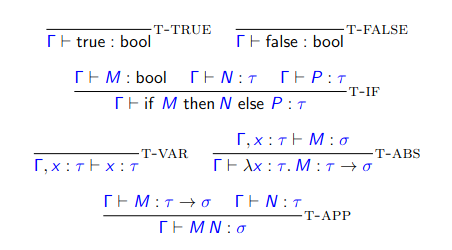
\includegraphics[scale=0.75]{reglas-tipado.png}
\end{center}

\teorema (Unicidad de tipos) \\
Si $\Gamma \vdash M : \tau$ y $\Gamma \vdash M : \sigma$ son derivable, entonces $\tau = \sigma$.

\demostracion supongo que $\Gamma \vdash M : \tau$ y $\Gamma \vdash M : \sigma$ pero $\tau \neq \sigma$.

Luego, $\exists T, S$ árboles de derivaciones de $\Gamma \vdash M : \tau$ y $\Gamma \vdash M : \sigma$ respectivamente.

Por inducción en cualquier árbol de derivación, veo que la elección de reglas es determinística porque hay exactamente un caso por constructor.

Luego, como en cada paso de la derivación se utilizan las mismas reglas y hay una única forma de aplicarlas veo que ambos árboles tienen la misma estructura.

Si en ambos árboles se llega a alguna aplicación de $T-VAR$ con una variable que deba tipar como $\tau$ en un árbol y como $\sigma$ en el otro, o algún tipo que los contenga, para que derive ambos casos debe pasar que para algún $x_i$, $(x_i : \tau) \in \Gamma$ y que $(x_i : \sigma) \in \Gamma$, pero como en $\Gamma$ no pueden haber variables repetidas, no puede ser el caso que se deriven ambos árboles, absurdo.

Si no, igualmente se puede ver por inducción en las reglas que los tipos que se deben satisfacer en cada paso son iguales menos el reemplazo $\tau$ por $\sigma$ y eventualmente se llega a $T-true$ ó $T-false$, en ambos casos terminé pidendo que en el caso base se satisfaga el tipo $bool$, osea el mismo tipo, con el caso base $T-var$ ya vimos que deben ser iguales, ahora mirando el árbol de arriba para abajo desde las hojas en cada paso los tipos son iguales y esta igualad de se mantiene hasta la raíz, absurdo por la supocición de que los tipos no coincidían. $\square$

\teorema (Weakening + Strenthening)
Si $\Gamma \vdash M : \tau$ es derivable y fv$(M) \subset$ dom$(\Gamma \cap \Gamma')$ entonces $\Gamma' \vdash M : \tau$ es derivable.

\demostracion construyo un árbol de derivación con la misma estructura pero reemplazando $\Gamma$ por $\Gamma'$ y por inducción en las reglas de derivación veo que todas siguen funcionando pues como pertenecen a fv$(M)$ no afectan ninguna regla.

% \subsection{Inferencia}

% \section{Prolog}
% \subsection{Reversibilidad}
%
% \section{SmallTalk}

\textit{Semántica operacional}
Indica cómo se ejecuta el programa hasta llegar a un resultada. Está la semántica small-step, ejecición paso a paso y la big-step, evaluación directa al resultado. Hay otros tipos de dar semántica formal como la semántica denotacional que interpreta los programas como objetos matemáticos y la semántica axiomática que establece relaciones lógicas entre el estado del programa antes y después de la ejecución. Vamos a trabajar con la semántica small-step.
\definicion un programa es un término $M$ tipable y cerrado (fv$(M) = \empty$). El juecio de tipado $\vdash M : \tau$ debe ser derivable para algún $\tau$.
\definicion juicios de evaluación. La semántica operacional predica sobre juicios de evaluación $M \rightarrow N$ donde $M$ y $N$ son programas.
\definicion los valores son los posibles resultados de evaluar programas:
$$ V::= true | false | \lambda x: \tau. M $$

\textit{Reglas de evaluación}
\begin{center}
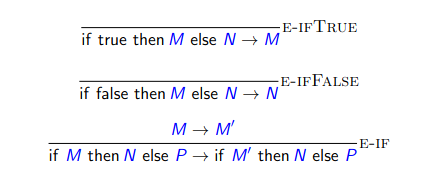
\includegraphics[scale=0.6]{reglas-sm1.png}
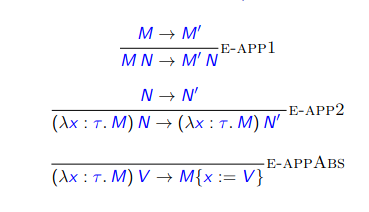
\includegraphics[scale=0.6]{reglas-sm2.png}
\end{center}

La operación de sustitución $M \{x := N\}$ denota el término que resulta de reemplazar todas las ocurrencias libres de $x$ en $M$ por $N$.

\begin{center}
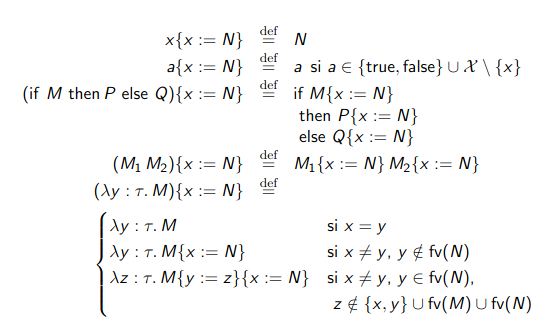
\includegraphics[scale=0.6]{sustitucion.png}
\end{center}

Definimos un juicio de evaluacion en muchos pasos $ M\rightarrow^* N$ donde $M$ y $N$ son programas.

\begin{center}
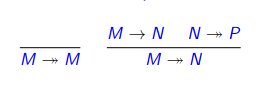
\includegraphics[scale=0.6]{reglas-sm3.png}
\end{center}

\subsubsection{Propiedades de la evaluación}

\teorema (Determinismo)
Si $M \rightarrow N_1$ y $M \rightarrow N_2$ entonces $N_1 = N_2$.

\teorema (Preservación te tipos)
Si $\vdash M : \tau$ y $M \rightarrow N$ entonces $\vdash N : \tau$.

\teorema (Progreso)
Si $\vdash M : \tau$ entonces o bien $M$ es un valor o bien existe $N$ tal que $M \rightarrow N$.

\teorema (Terminación)
Si $\vdash M : \tau$, entonces no hay una cadena infinita de pasos $M \rightarrow M_1 \rightarrow M_2 \rightarrow ...$

\corolario (Canonicidad)

\begin{enumerate}
\itemsep-0.35em 
\item Si $\vdash M : bool$ es derivable, entonces la evaluación de $M$ termina y el resultado es true o false.
\item Si $\vdash M : \tau \rightarrow \sigma$ es derivable, entonces la evaluación de $M$ termina y el resultado es una abstracdción.
\end{enumerate}

\subsubsection{Cálculo-$\lambda^bn$}
Es una extensión del cálcula lambda, mirar las diapos
Un programa $M$ está en forma normal (f.n.) si no existe $M'$ tal que $M \rightarrow M'$.

Que una fórmula sea cerrada y tipable no implica que sea un valor a diferencia del cálculo-$\lambda^b$

Las f.n.'s que no son valores se llamas términos de error.

\subsection{Inferencia}
\textit{Términos sin anotaciones de tipos}
$$ U ::= x | \lambda x. U | U U | \text{True} | \text{False} | \text{if } U \text{ then } U \text{ else } U $$
\textit{Términos con anotaciones de tipos}
$$ M ::= x | \lambda x: \tau. U | U U | \text{True} | \text{False} | \text{if } U \text{ then } U \text{ else } U $$
\definicion notamos erase($M$) al término sin anotaciones de tipos que resulta de borrar las anotaciones de tipos de $M$
\definicion un término $U$ sin anotaciones de tipos es tipable sii existe un contexto tipado $\Gamma$, un término con anotaciones de tipos $M$ y un tipo $\tau$ tales que $\text{erase}(M) = U$ y $\Gamma \vdash M : \tau$.

\textit{Problema de inferencia de tipos}. Consiste en dado un término $U$, determinar si es tipable. En caso de que lo sea, hallar $\Gamma, M, \tau$ tales que cumplan la definición de tipado.

\textit{Algoritmo $I$}
El algoritmo $I$ recibe un término $U$ sin anotaciones de tipos. Conta de cuatro pasos.

\subsubsection{Rectificación}
Decimos que un término está rectificado si no hay dos variables ligadas con el mismo nombre y no hay una variables ligada con el mismo nombre que una libre. Siempre se puede rectificar un término $\alpha$-renombrándolo.

\subsubsection{Anotación}
Tenemos un término $U$, que suponemos ya rectificado. Producimos un contexto $\Gamma_0$ que le da tipo a todas las variables libres de $U$ con una incógnita fresca y un término $M_0$ que está anotado de tal modo que erase$(M_0) = U$ con incógnitas frescas.

\subsubsection{Generación de restricciones}
Tenemos un contexto $\Gamma$ y un término $M$ con anotaciones de tipos. Recursivamente calculamos un tipo $\tau$ que corresponde al tipo de $M$ y un conjunto de ecuaciones $E$ que representan restricciones para que $M$ esté bien tipado.

Definimos un algoritmo recursivo $I(\Gamma | M) = (\tau | E)$ con la precondición de que $\Gamma$ le da tipo a todas las variables libre de $M$.

$I(\Gamma | \True) = (\Bool | \emptyset )$ \\
$I(\Gamma | \False) = (\Bool | \emptyset)$ \\
$I(\Gamma | x) = (\tau | \emptyset)$ si $(x: \tau) \in \Gamma$ \\
$I(\Gamma | \ifelse{M_1}{M_2}{M_3} = (\tau_2 | \{\tau_1 \equ \Bool, \tau_2 \equ \tau_3\} \cup E_1 \cup E_2 \cup E_3)$ \\
donde $I(\Gamma | M_1) = (\tau_1 | E_1)$, $I(\Gamma | M_2) = (\tau_2 | E_2)$, $I(\Gamma | M_3) = (\tau_3 | E_3)$ \\
$I(\Gamma | M_1 M_2) = (X_k | \{\tau_1 \equ (\tau_2 \rightarrow X_k)\} \cup E_1 \cup E_2$ \\
donde $I(\Gamma | M_1) = (\tau_1 | E_1)$, $I(\Gamma | M_2) = (\tau_2 | E_2)$ \\
$I(\Gamma | \lambda x : \tau. M) = (\tau \rightarrow \sigma | E)$ \\
donde $I(\Gamma, x : \tau | M) = (\sigma | E)$

\subsubsection{Unificación}
Una vez calculado $I(\Gamma_0 | M_0) = (\tau | E)$, calculamos $S = \text{mgu}(E)$, si no existe, el término $U$ no es tipable, si existe, el término $U$ es tipable y vale $S(\Gamma_0) \vdash S(M_0) : S(\tau)$.

\end{document}
